% !TEX root = mythesis.tex

%==============================================================================
\chapter{The \tZqsec production}
\label{sec:tZq}
%==============================================================================

The proton-proton collisions occurring at high energies at the LHC allow 
multiple processes that produce heavy particles. One of these
processes is the electroweak production of the \Ptop-quark and the 
\PZ-boson. As shown in \cref{fig:tZqfeyna}, 

In this analysis, this production
is referred to as the \tZq production described by Feynman diagrams in 
\cref{fig:tZqfeyn}. 

\begin{figure}[htbp]
    \centering
    \begin{subfigure}{0.35\figwidth}
      \centering
         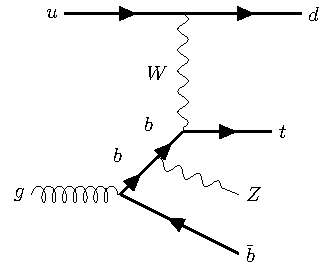
\includegraphics[width=\textwidth]{tZq_Zfromb.pdf}
         \label{fig:tZqfeyna}
    \end{subfigure}
    \qquad
    \begin{subfigure}{0.35\figwidth}
      \centering
      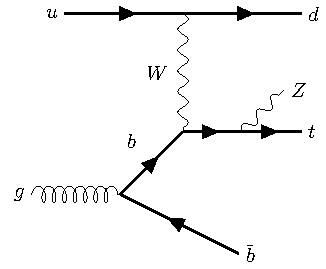
\includegraphics[width=\textwidth]{tZq_Zfromtop.pdf}
      \label{fig:tZqfeyn(b)}
    \end{subfigure}
    \begin{subfigure}{0.35\figwidth}
      \centering
      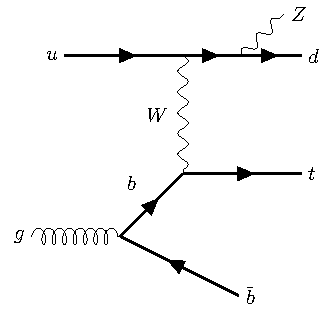
\includegraphics[width=\textwidth]{tZq_Zfromd.pdf}
      \label{fig:tZqfeyn(c)}
    \end{subfigure}
  
  
  \medskip
  
  
  \begin{subfigure}{0.35\figwidth}
      \centering
      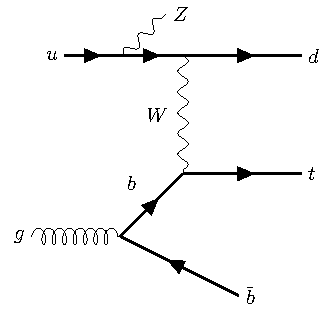
\includegraphics[width=\textwidth]{tZq_Zfromu.pdf}
    \end{subfigure}
    \begin{subfigure}{0.35\figwidth}
      \centering
      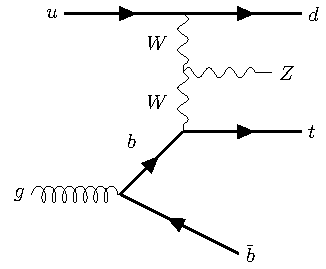
\includegraphics[width=\textwidth]{tZq_ZfromWW.pdf}
    \end{subfigure}
    \begin{subfigure}{0.35\figwidth}
        \centering
        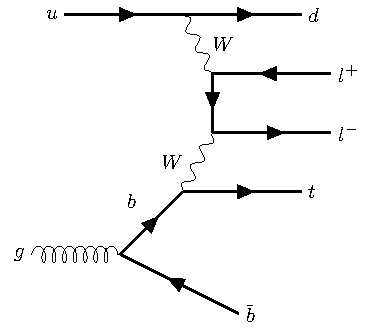
\includegraphics[width=\textwidth]{tZq_nonres.pdf}
      \end{subfigure}
  
  \caption[Feynman diagrams at LO for the \tZq-process]{Feynman diagrams at 
  LO for the \tZq-process. The \PZ is radiated either from incoming or 
  outgoing quarks or from the exchanged W boson. }
  \label{fig:tZqfeyn}
  \end{figure}

\mynote[inline]{}{The s-channel t-channel resonance non-resonance diagram 
explanation.}

The \tZq production is interesting to study because it probes the coupling
of fermion-fermion and fermion-boson simultaneously. Moreover, it can provide
a solid basis to study the even rarer $tHq$ process. It is important to note 
that the particles involved in this production are quite heavy and therefore,
the only way to spot them is by reconstructing their decay products. 
Conventionally, the decay products are divided into several \textit{channels}
based on certain combination of leptons and jets. This analysis is based on
the so-called trilepton channel.

\section{The \tZqsec Trilepton Channel}
As the name suggests, the trilepton decay channel of the \tZq production 
contains mainly three leptons. The probability of having three leptons in 
the final state is very small. However, the leptons allow for a clean signature
of this channel and therefore, \tZq is studied in the trilepton channel. This
will be referred to as the signal.

The list of objects belonging to this decay channel can be obtained from its
Feynman diagram as shown in FIGURE. It also helps in generating certain
criteria to extract these objects from the entire reconstructed data.
This procedure is called event selection. For this specific channel, the
event selection consists of three leptons that must originate either 
from \PZ or from \PW which is decaying from \Ptop. Moreover, 
there should be at least one \Pbottom-jet from \Ptop along with
missing transverse energy. In addition, the spectator quark should 
also be considered through a condition on number of jets. 
The event selection is summarised in TABLE. Along with the number of leptons
and jets, requirements are also placed on their kinematic properties in the
form of cuts on their transverse momenta and eta. 

It is important to note here that, these requirements are chosen to 
maximise the probablility of selecting signal events
but in reality there are background processes that mimic the \tZq signature
and therefore, contaminate the selected signal data. 


\begin{table}[!htbp]
    \footnotesize
    \caption{Definition of the signal and control regions.}
    \label{tab:selection:srcr}
    \renewcommand{\arraystretch}{1.3}
    \centering
    \begin{tabular}{lccc}
        \toprule
        Variable & \multicolumn{3}{c}{Preselection}\\
        \midrule
        $N_\ell~\left(\ell=e,\mu\right)$ & \multicolumn{3}{c}{$=3$}\\
        & \multicolumn{3}{c}{$\ge 1$ OSSF lepton pair}\\
        $\pT\left(\ell_1,\ell_2,\ell_3\right)$ & \multicolumn{3}{c}{$>$ 27,~15, \qty{10}{\GeV}}\\
        Sum of lepton charges & \multicolumn{3}{c}{$\pm 1$}\\
        $\min(m_{\ell\ell})$ & \multicolumn{3}{c}{$>$ \qty{20}{\GeV}} \\
        $|m_{\ell\ell} - m_{Z}|$ & \multicolumn{3}{c}{$<$ \qty{10}{\GeV}} \\
        \mtw & \multicolumn{3}{c}{$>$ \qty{30}{\GeV}} \\
        \midrule
        & SR & \CRttZ & \CRVV \\
        $N_\text{jets}\left(\pT>25~\mathrm{GeV}\right)$ & 2-5 & $\ge 6$ & 2-5 \\
        $N_{b-\text{jets}} @ 85\%$ & 1-2 (no $2j2b$) & $\ge 1$ & 0 \\
        \bottomrule
    \end{tabular}
    \end{table}


\section{Background processes}
